\documentclass{article}

\usepackage{amsmath}
\usepackage{amssymb}
\usepackage[backend=bibtex, style=authoryear]{biblatex}
\addbibresource{refs.bib}
\usepackage{graphicx}
\usepackage{verbatim}
\usepackage{subcaption}

\author{Valentin Vogelmann}

\title{Theoretically Sound Estimation of Zipf's Law}

\begin{document}
\maketitle

Reminder: In his review of Zipf's law, \parencite{piantadosi2014zipf} noticed an important methodological issue in the common way of estimating it (i.e. estimating rank and frequency of a word): If the ranks of words are calculated from the frequencies obtained from a corpus, then 
the resulting relationship contains spurious regularity. As a solution, \parencite{piantadosi2014zipf} proposed using $f' \sim Binom(n=f, p=0.5)$, where $f$ is the frequency observed in a corpus, and $r = f - f'$ as estimates for frequency and rank, respectively. Note that this is equivalent to randomly sampling words from a corpus for the frequency estimate and using the rest of the corpus for the rank estimate. The proposed technique removes the statistical dependence between rank and frequency, and allows for interpretation of persisting regularities, such as patterns in statistical error. Indeed, the author found a strong autocorrelation in the error of the maximum likelihood estimate of Zipf's law when using the newly proposed estimation technique.\\

This summary reproduces these results in multiple languages with the use of Wikipedia, and strengthens them by removing an issue in the solution of \parencite{piantadosi2014zipf}: Randomly dividing a corpus will still lead to bias in the estimates because the sequential structure of language is not uniform. For instance, \parencite{corral2009universal} have found complex distributions over interappearance distances of word tokens of the same types, indicating that sampling words from corpora at constant, uniform rates provides biased frequency estimates. Eventually, one has to use two independent corpora with the same domains to obtain independent and unbiased estimates of ranks and frequencies. The article-based structure of Wikipedia offers a convenient solution for this issue: Articles are to a large degree independent from each other in the sense that occurrences of words do not influence each other across articles but are similar in language. Hence, instead of randomly sampling words, we randomly sample articles, creating two independent but linguistically faithful subcorpora from which we can estimate ranks and frequencies of words.

\section{Data: Wikipedia}

\subsection*{Languages}

\begin{itemize}
\item Arabic (AR)
\item Esperanto (EO)
\item Basque (EU)
\item Finnish (FI)
\item Indonesian (ID)
\item (Japanese (JA))
\item (Korean (KO))
\item Norwegian (NO)
\item Turkish (TR)
\item Vietnamese (VI)
\end{itemize}

This selection is mainly based on size of the Wikipedias and on the morphological properties and relatedness-status of the languages. Japanese and Korean have not been included in the analyses yet for lack of appropriate tokenisers.\\
 % Arabic (Semitic) has a unique root-based morphology; Esperanto is a constructed language; Basque, Japanese, Korean are language isolates (at least not realted to any other macro-families); Finnish, Japanese, Korean, Turkish have agglutinative morphology; Vietnamese has isolating morphology; Basque makes an ergative-absolutive distinction; Indonesian is mainly a lingua franca; Norwegian is a member of the Indo-European family; Turkish is a member of the Turkic family. Arabic, Korean, and Japanese do not use Latin-based writing systems, and out of lack for tokenisers for Korean and Japanese, these have not been part of the analyses yet.

\subsection{Methods}

The Wikimedia periodically creates complete dumps of all Wikipedias that are used for back-up and are made publicly available (\verb|https://dumps.wikimedia.org/|). These dumps contain Wikipedia-specific XML code but since we are only interested in the text, we use the Python-based WikiExtractor \parencite{WikiExtractor} that removes all annotations as well as tables, headers, and links and returns paragraph-separated plain text. For tokenisation, we require high robustness across languages and fast performance for which the TokTokTokenizer module \parencite{dehdari2014neurophysiologically} contained in the nltk Python library seems to be a good choice. After tokenisation, we remove punctuation and special characters for which there is unfortunately no principled cross-linguistic method. The current set of characters to be removed is based on dedicated code-blocks in the Unicode specification (e.g. the punctuation section in the Basic Latin block and the CJK Symbols and Punctuation block).\\

As described above, we randomly sample the articles of each Wikipedia into two subcorpora for estimation of ranks and frequencies. In addition, we randomly sample paragraphs (subelements of articles), and words (subelements of paragraphs) the latter of which corresponds to the method of \parencite{piantadosi2014zipf}. Using the different levels of splitting is intended for reproducing the previous results and for exposing and making interpretable any biases that arise from sampling at the word level. 



\subsection{Basic Statistics}

\begin{table}[ht]
	\def\arraystretch{1.25}
	\centering
	\makebox[\textwidth]{
		\begin{tabular}{c|r r r r r r r r}
			& AR & EO & EU & FI & ID & NO & TR & VI\\\hline
			Articles & 565559 & 244990 & 288364 & 430864 & 422461 & 482595 & 300415 & 1162556\\
			Paragraphs & 2385848 & 994419 & 1133763 & 1925574 &  1563794 & 1972020 & 1425438 & 2408102\\
			Tokens & 92825514 & 38239150 & 31225987 & 73633412 & 63800296 & 85688201 & 53744489 & 116597143\\
			Types & 2174113 & 1181503 & 838297 & 3007242 & 893553 & 1702145 & 1249304 & 984833\\\vspace{0.5em}
			Type-Token Ratio & 0.023 & 0.031 & 0.027 & 0.041 & 0.014 & 0.019 & 0.023 & 0.008\\
			Types in Intersection &681170 & 358082&275774&958797&283631&549819&438015&286743 \\\vspace{0.5em}
			(\% of Types) & 0.313 & 0.303 & 0.329 & 0.319 & 0.317 & 0.323 & 0.351 & 0.291\\
			Tokens in Intersection &90825718&37112604&30420953&70835274&62843389&84081221&52595422&115596836\\
			(\% of Tokens) & 0.978 & 0.971 & 0.974 & 0.962 & 0.985 & 0.981 & 0.979 & 0.991\\
		\end{tabular}}
		\label{Wiki}
		\caption{Basic Statistics from the Wikipedias; see above for the language codes.}
	\end{table}


In table 1, "Types in Intersection" refers to the number of word types in the intersection of the frequency and the rank subcorpora, "Tokens in Intersection" then refers to the number of tokens of these types in the intersection. These are the effective numbers for all analyses, since those word types that did not occur in both of the two subcorpora are removed for the estimation of Zipf's law. "Types in Intersection" displays the values for the splitting level of articles. The values for the level of paragraphs and the level of words are higher, each by around 10\% consistently across languages. "Tokens in Intersection" also displays the values for the level of articles, but the values of the levels of words and paragraphs are the same (within 99\% of each other).

The percentages of "Types in Intersection" and "Tokens in Intersection" show the clear effect of sampling under the regime of Zipf's law: while only around 30\% of word types were preserved after intersecting two randomly sampled subcorpora, almost all word tokens were captured. This exactly mirrors the Zipfian distribution over word types in which most word types are very infrequent and few most frequent word types constitute the majority of any corpus. Remarkably, this relationship is very stable across languages, and seems to vary with the type-token ratio.




\section{Comparing the Splitting Levels}

Based on the above observations, the three levels of splitting (namely articles, paragraphs, and words) are expected to yield quite different results when used to estimate Zipf's law. Specifically, splitting on the level of articles is expected to best preserve the complex structure of language and hence produce more deviation from Zipf's law. Moreover, the deviation is expected to be more patterned, reflecting the fact that words are not randomly sampled into text but following highly specific patterns.\\

\begin{figure}
	\centering
	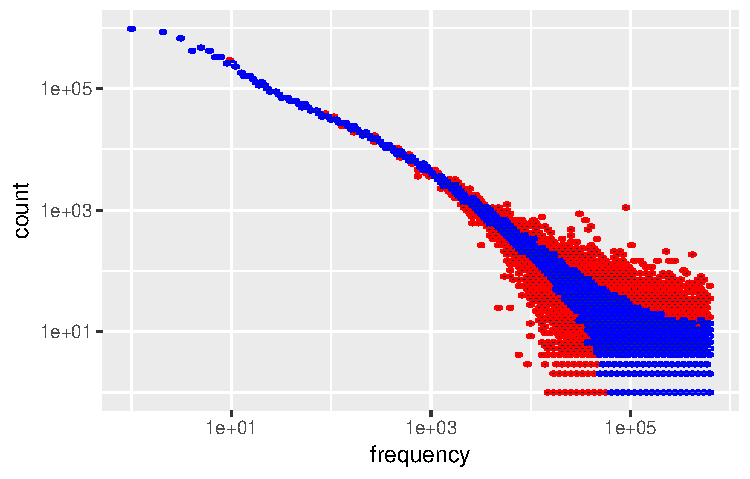
\includegraphics[scale=0.8]{ID-levels-overlay.pdf}
	\caption{Rank-frequency for Indonesian plot of two splitting levels: article (red), and word (blue) superimposed.}
	\label{levels-overlay}
\end{figure}


Surprisingly, this does not quite turn out to be the case. While splitting at the level of articles does result in greater deviation from Zipf's law, this only affects low-frequency words which naturally have high variance on all splitting levels. Figure \ref{levels-overlay}, which displays the word-level frank-frequency plot superimposed on the article-level rank-frequency plot, shows this trend which is again remarkably robust across languages. Especially for higher-frequency words, the estimates converge entirely, displaying the same structure in the deviation from Zipf's law. This is also clear from figure \ref{levels-correl} which plots the correlation between frequency estimates obtained from article-level splitting and frequency estimates from word-level splitting. Correlation only deteriorates when frequencies become smaller which is natural since those estimates have high intrinsic variance. Finally, plotting the empirical cumulative distribution functions of the three splitting levels again shows divergence in the low frequencies, specifically that word-level splitting leads to more word types with low frequencies.\\

\begin{figure}
	\centering
	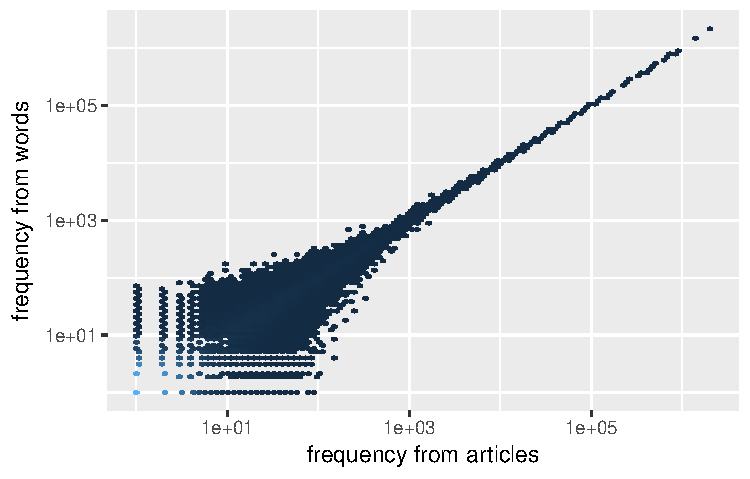
\includegraphics[scale=0.8]{NO-count-count-corr.pdf}
	\caption{This plot relates the frequency estimates from article-level splitting (horizontal) to the estimates from word-level splitting (vertical). The language used is Norwegian.}
	\label{levels-correl}
\end{figure}


A possible explanation of these observations, namely high similarity between the estimates from the different splitting levels but higher variance in low-frequency levels for article-level splitting, relies on the topicality of words: high-frequency words are typically uniformly distributed across articles and paragraphs, indicating low topicality (see e.g. \parencite{serrano2009beyond} for an analysis on distribution across documents and topicality). This implies similar likelihoods of being sampled in article-level splitting and in word-level splitting. Low-frequency words, on the other hand, are typically highly topical and in extreme cases only appear in a single article. Such a case leads to high deviance from Zipf's law as the word will be assigned high rank but low frequency (or vice-versa). Sampling on the level of words avoids this by keeping the probability of sampling such a highly topical constant across instances. It remains an open question, however, to what extent the results found here depend on corpus size, and whether the results obtained from the different levels of splitting diverge to larger a larger extent with smaller corpus sizes.\\

Regardless of the high similarity between the word-level splitting estimates and the article-level splitting estimates, we know that word-level splitting has methodological issues and that article-level estimation gives an image of Zipf's law that is more faithful to linguistic structure. The results found here thus add to stances like that of \parencite{piantadosi2014zipf} that Zipf's law is remarkably robust in language but that the substantial divergence from cannot be neglected either. Specifically, with the new results obtained from article-level estimation, the divergence is greater than previously assumed, even with very large data sizes. 


\begin{figure}
	\centering
	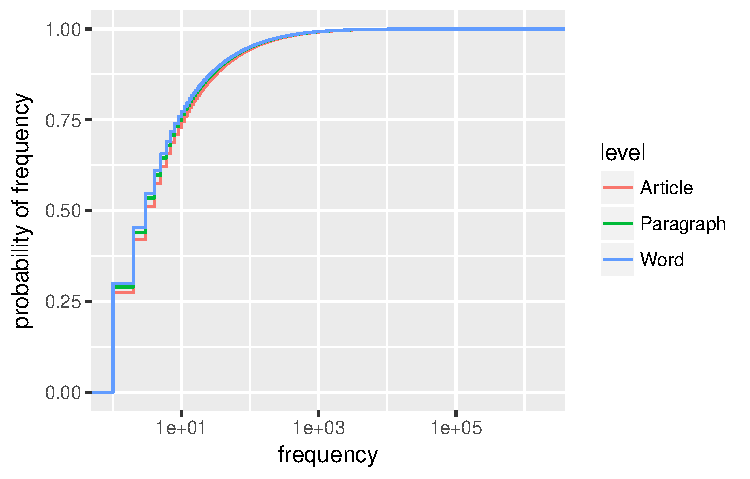
\includegraphics[scale=0.9]{AR-ecdf.pdf}
	\caption{The empirical cumulative distribution functions of the three splitting levels obtained from Arabic. This is the distribution over the frequency of a word type, e.g. slightly over 25\% of word types have frequency 1.}
	\label{ECDFS}
\end{figure}





\section{Zipf's Law}


\begin{figure}
	\centering
	\begin{subfigure}[b]{0.3\textwidth}
		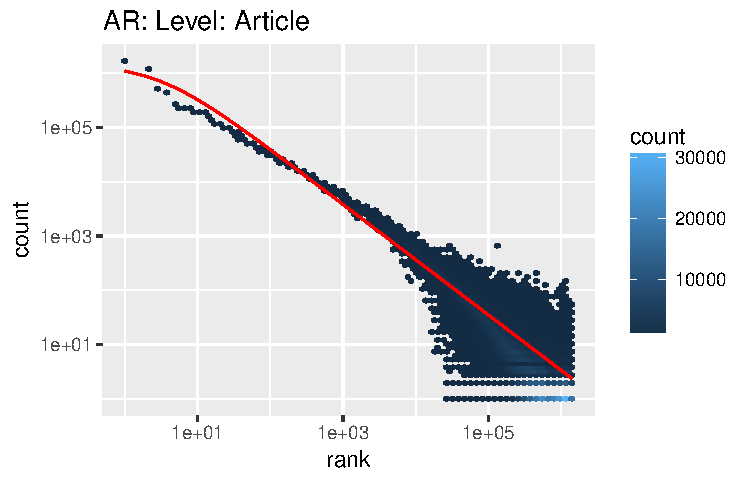
\includegraphics[trim={0 0 2.2cm 0.6cm},clip, width=\textwidth]{AR_Article_mle.pdf}
		\caption{Arabic}
		\label{fig:ar_mle}
	\end{subfigure}
	~ %add desired spacing between images, e. g. ~, \quad, \qquad, \hfill etc. 
	%(or a blank line to force the subfigure onto a new line)
	\begin{subfigure}[b]{0.3\textwidth}
		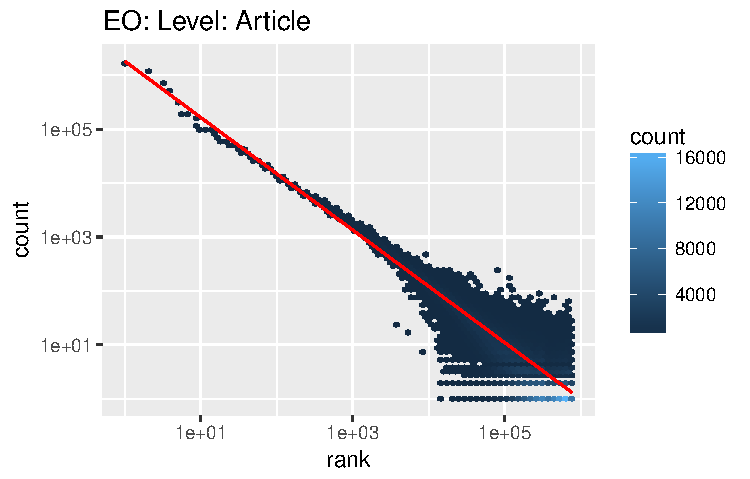
\includegraphics[trim={0 0 2.2cm 0.6cm},clip, width=\textwidth]{EO_Article_mle.pdf}
		\caption{Esperanto}
		\label{fig:eo_mle}
	\end{subfigure}
	~ %add desired spacing between images, e. g. ~, \quad, \qquad, \hfill etc. 
	%(or a blank line to force the subfigure onto a new line)
	\begin{subfigure}[b]{0.3\textwidth}
		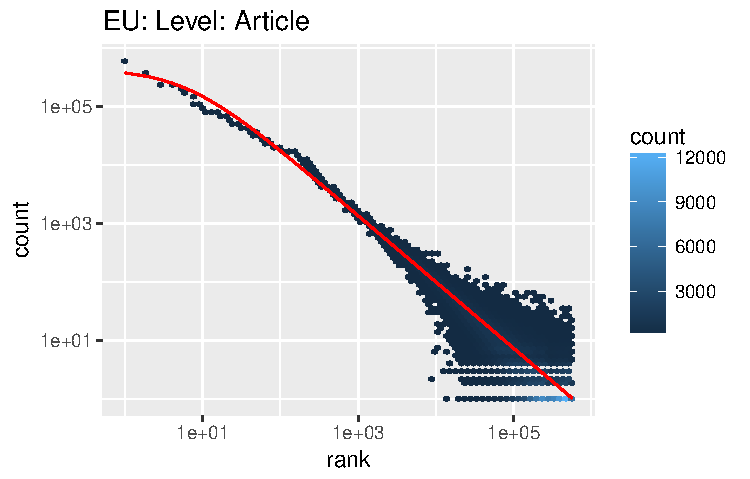
\includegraphics[trim={0 0 2.2cm 0.6cm},clip, width=\textwidth]{EU_Article_mle.pdf}
		\caption{Basque}
		\label{fig:eu_mle}
	\end{subfigure}
	
	\begin{subfigure}[b]{0.3\textwidth}
		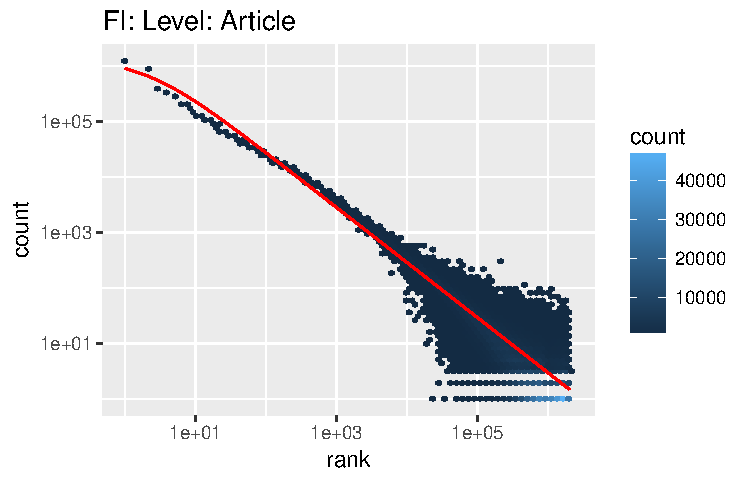
\includegraphics[trim={0 0 2.2cm 0.6cm},clip, width=\textwidth]{FI_Article_mle.pdf}
		\caption{Finnish}
		\label{fig:fi_mle}
	\end{subfigure}
	~ %add desired spacing between images, e. g. ~, \quad, \qquad, \hfill etc. 
	%(or a blank line to force the subfigure onto a new line)
	\begin{subfigure}[b]{0.3\textwidth}
		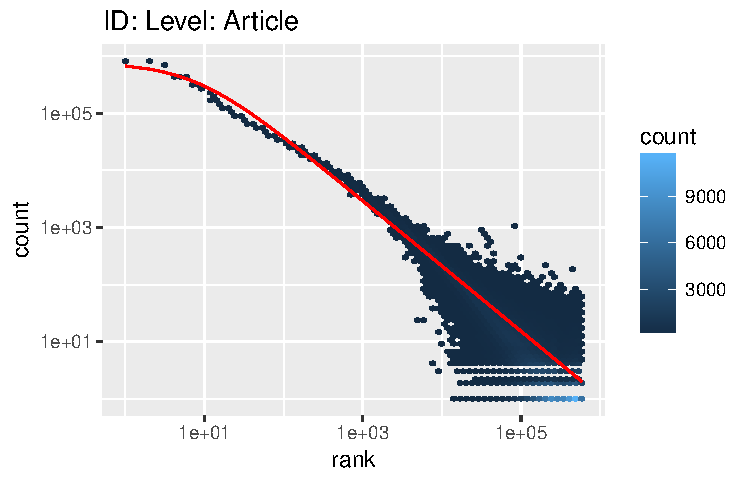
\includegraphics[trim={0 0 2.2cm 0.6cm},clip, width=\textwidth]{ID_Article_mle.pdf}
		\caption{Indonesian}
		\label{fig:id_mle}
	\end{subfigure}
	~ %add desired spacing between images, e. g. ~, \quad, \qquad, \hfill etc. 
	%(or a blank line to force the subfigure onto a new line)
	\begin{subfigure}[b]{0.3\textwidth}
		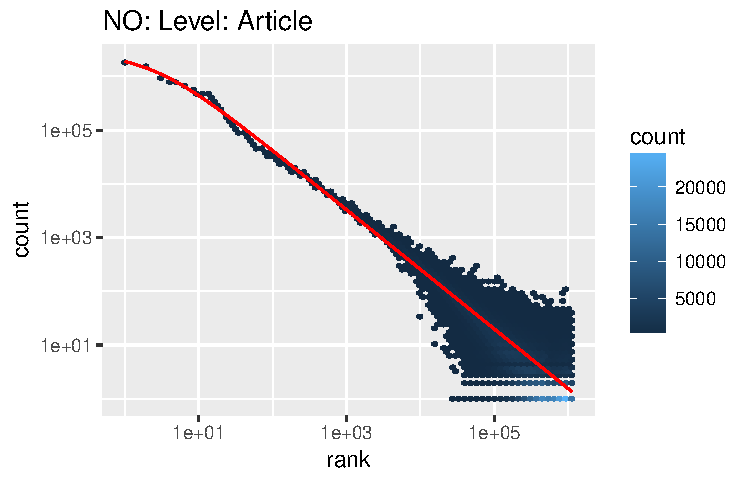
\includegraphics[trim={0 0 2.2cm 0.6cm},clip, width=\textwidth]{NO_Article_mle.pdf}
		\caption{Norwegian}
		\label{fig:no_mle}
	\end{subfigure}
	
	\begin{subfigure}[b]{0.3\textwidth}
		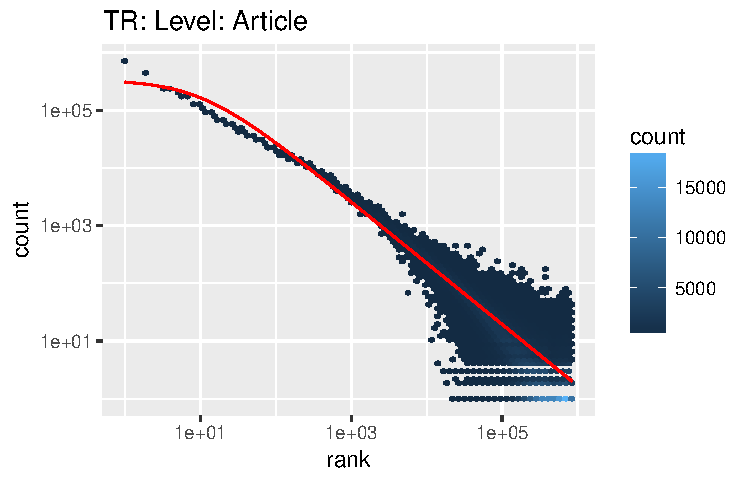
\includegraphics[trim={0 0 2.2cm 0.6cm},clip, width=\textwidth]{TR_Article_mle.pdf}
		\caption{Turkish}
		\label{fig:tr_mle}
	\end{subfigure}
	~ %add desired spacing between images, e. g. ~, \quad, \qquad, \hfill etc. 
	%(or a blank line to force the subfigure onto a new line)
	\begin{subfigure}[b]{0.3\textwidth}
		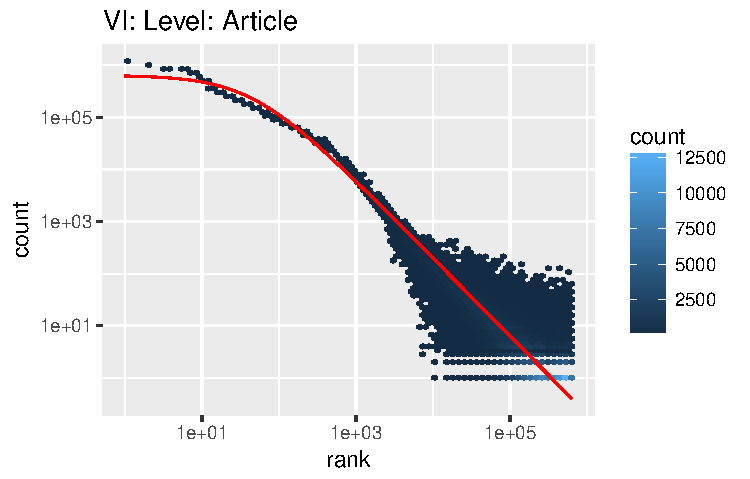
\includegraphics[trim={0 0 2.2cm 0.6cm},clip, width=\textwidth]{VI_Article_mle.pdf}
		\caption{Vietnamese}
		\label{fig:vi_mle}
	\end{subfigure}
	\caption{Rank-frequency plots (blue hexagons) with the Mandelbrot maximum likelihood estimates (red).}
	\label{fig:mles}
\end{figure}

\subsection{Estimation \& Results}

Following \parencite{piantadosi2014zipf} we do not estimate Zipf's law itself which only ha a single free parameter: $f(w_r) \propto r^{-\alpha}$. Instead, we estimate Mandelbrot's law, $f(w_r) \propto (r + \beta)^{-\alpha}$, which has two free parameters, and hence allows for better fit. The purpose of the parameter $\beta$ is to allow the empirical law to have curvature in the high-frequency ranges but its effect vanishes as the rank $r$ increases.\\

Figure \ref{fig:mles} contains the rank-frequency plots for the eight languages we analysed. All estimates were obtained from splitting Wikipedia on the level of articles, thus the high variance in the low-frequency ranges of the plots. As already hinted at above, remarkably, the structured deviation in the higher-frequency ranges (where the variance is considerably decreased) survives article-level splitting. The red lines in the plots show the maximum likelihood estimates of the parameters $\alpha$ and $\beta$ in Mandelbrot's law, estimated from the same datasets in the plots. The parameters' values are given in table \ref{params}. 


\begin{table}[ht]
\centering
\begin{tabular}{c|c c c c c c c c }
	& AR & EO & EU & FI & ID & NO & TR & VI\\\hline
	$\alpha$ & 1.02 & 1.04 & 1.14 & 0.99 & 1.14 & 1.11 & 1.06 & 1.49  \\
	$\beta$ &  2.89 & -0.00 & 6.05 & 2.00 & 7.63 & 2.22 & 10.17 & 45.06  \\
\end{tabular}
	\caption{Maximum likelihood estimates for parameters $\alpha$ and $\beta$ of Mandelbrot's law.}
	\label{params}
\end{table}


\begin{comment}

\subsection{Error}

\subsubsection{Random Baseline}

In order to check the meaningfulness in the error structure we obtain from the corpora, we perform the same analyses on a random baseline. This baseline is constructed by constructing a sequence of words randomly drawn from a Mandelbrot distribution. The parameters for the basic random baseline are $\alpha=1$ and $\beta=2$ which are common values found empirically.\\
We then perform an MLE on the parameters $\alpha$ and $\beta$ of the Mandelbrot model, and compute $error_r = \log(\frac{theoretical.prob_r}{empirical.prob_r})$ for each rank $r$, just as with the empirical data.\\\\
With respect to the randomly drawn data, the MLE of $\alpha$ and $\beta$, and $error_r$, we expect the following:\\
The MLE should return the true parameters, since the model is also the true model from which the data was generated.\\
The distribution of the error should have mean and mode 0 and should be symmetric.\\
There should be no autocorrelation in the error, i.e. the error of rank $r+\tau$ should not be correlated with the error of $r$ (where $\tau = 1$ is the lag).\\
In summary, the error of the random baseline should be random to extent that the Mandelbrot model is random (note that for high ranks, there will be substantially more variance in the error due to low counts).
\end{comment}


\newpage
\nocite{*}
\printbibliography
\end{document}